\documentclass[a4paper, 12pt]{article}
%\documentclass{book}

% Important Packages:
 \usepackage{amsmath}    % need for subequations
 \usepackage{amsfonts}
 \usepackage{amsthm}
 \usepackage{graphicx}   % need for figures
 \usepackage{verbatim}   % useful for program listings
 \usepackage{tikz,tkz-euclide}
 \usepackage{amssymb}
 
 \usetikzlibrary{calc,patterns,angles,quotes}
\usetkzobj{all}

\def\deg{^{\circ}}
\newcommand\heading[1]{\ \\\large{\textbf{#1}}}
\newcommand\ora[1]{\overrightarrow{#1}}

\def\thm{Th\textsuperscript{\underline{m}}}

%------------------end---preamble--------------------
 
 % Useful macros 
 \def\tcb#1{\color{blue}{#1}}
 \def\tcr#1{\color{red}{#1}}	
 \def\tcg#1{\color{green}{#1}}
 \def\be{\begin{eqnarray}}	 	\def\ee{\end{eqnarray}}
 \def\bea{\begin{eqnarray}}	 	\def\eea{\end{eqnarray}}
 \def\bean{\begin{eqnarray*}}	\def\eean{\end{eqnarray*}}
 
 \def\D{\displaystyle}
 \def\T{\textstyle}
 \def\l{\left}
 \def\r{\right}
 \def\nf{n_{\!f}} % quark flavours
 \def\pa{\partial}
 \def\eg{e.\,g.}
 \def\ie{i.\,e.}

 \def\be{\begin{equation}}
 \def\ee{\end{equation}}
 \def\bea{\begin{eqnarray}}
 \def\eea{\end{eqnarray}}
 \def\bean{\begin{eqnarray*}}
 \def\eean{\end{eqnarray*}}
 \def\gsim{\mathrel{\rlap{\lower0.2em\hbox{$\sim$}}\raise0.2em\hbox{$>$}}}
 \def\ksim{\mathrel{\rlap{\lower0.2em\hbox{$\sim$}}\raise0.2em\hbox{$<$}}}
 \def\kg{\mathrel{\rlap{\lower0.25em\hbox{$>$}}\raise0.25em\hbox{$<$}}}
 
 \def\AA{${\buildrel_{\circ} \over {\mathrm{A}}}$}
 \def\bm#1{\mbox{\boldmath$#1$}}
 \newcommand{\eq}[1]{(\ref{#1})} 
 \def\pd{\partial}
 \def\d{\textrm{d}} 
 \def\T{\textstyle}
 \def\eg{e.\,g.}	% exempli gratia (for the sake of example)
 \def\ie{i.\,e.}	% id est (that is)


 % Page configuration:
 \topmargin -2.0cm
 \oddsidemargin -0.85cm
 \evensidemargin -0.85cm
 \textwidth 18cm
 \textheight 24cm
 
\begin{document}
\begin{center}
\textbf{April Camp 2019 \\ Senior Test 2} \\
\textbf{Solutions}
\end{center}
\vspace{5mm}

\begin{enumerate}

%  2018 shortlist C1
\item[1.]  \textit{Let $n \geq 3$ be an integer. Prove that there exists a set $S$ of $2n$ positive integers satisfying the following property: For every $m = 2, 3, \dots, n$ the set $S$ can be partitioned into two subsets with equal sums of elements, with one of the subsets of cardinality $m$.
}
\vspace{5mm}


\textbf{Solution:}  We show that one of the possible examples is the set
$$
S = \{ 1 \cdot 3^k, 2 \cdot 3^k, k = 1, 2, \dots, n-1 \} \cup \left\{  1, \frac{3^n + 9}{2} - 1  \right\}
$$
It is readily verified that all the numbers listed above are distinct (notice that the last two are not divisible by 3).

The sum of elements in $S$ is
$$
\Sigma = 1 +  \left( \frac{3^n + 9}{2} - 1 \right)  + \sum_{k=1}^{n-1} (1 \cdot 3^k + 2 \cdot 3^k ) = \frac{3^n + 9}{2} + \sum_{k=1}^{n-1} 3^{k+1} = \frac{3^n + 9}{2} + \frac{3^{n+1} - 9}{2} = 2 \cdot 3^n
$$

Hence, in order to show that this set satisfies the problem requirements, it suffices to present, for every $m = 2, 3, \dots, n$, an $m$-element subset $A_m \subset S$ whose sum of elements equals $3^n$.

Such a subset is
$$
A_m = \{2 \cdot 3^k : k = n-m+1, n-m+2, \dots, n-1 \} \cup \{1, 3^{n-m+1} \}.
$$

Clearly, $|A_m| = m$. The sum of elements in $A_m$ is
$$
3^{n-m+1} + \sum_{k=n-m+1}^{n-1} 2 \cdot 3^k = 3^{n-m+1} + \frac{2 \cdot 3^n - 2 \cdot 3^{n-m+1}}{2} = 3^n,
$$
as required.  \qed

\vspace{5mm}
\textbf{Comment: }  Let us present a more general construction. Let $s_1, s_2, \dots, s_{2n-1}$ be a sequence of pairwise distinct positive integers satisfying $s_{2i+1} = s_{2i} + s_{2i-1}$ for all $i = 2, 3, \dots, n-1$. Set $s_{2n} = s_1 + s_2 + \dots + s_{2n-4}$. \\

Assume that $s_{2n}$ is distinct from the other terms of the sequence. Then the set $S = \{s_1, s_2, \dots, s_{2n} \}$ satisfies the problem requirements. Indeed the sum of its elements is
$$
\Sigma = \sum_{i=1}^{2n-4} s_i + (s_{2n-3} + s_{2n-2}) + s_{2n-1} + s_{2n} = s_{2n} + s_{2n-1} + s_{2n-1} + s_{2n} = 2s_{2n} + 2s_{2n-1}.
$$

Therefore, we have
$$
\frac{\Sigma}{2} = s_{2n} + s_{2n-1} = s_{2n} + s_{2n-2} + s_{2n-3} = s_{2n} + s_{2n-2} + s_{2n-4} + s+{2n-5} = \dots
$$
which shows that the required set $A_m$ can be chosen as
$$
a_m = \{ s_{2n}, s_{2n-2}, \dots, s_{2n-2m+4}, s_{2n-2m-3} \}.
$$

So, the only condition to be satisfied is $s_{2n} \not \in \{s_1, s_2, \dots, s_{2n-1} \}$, which can be achieved in many different ways (e.g., by choosing properly the number $s_1$ after specifying $s_2, s_3, \dots, s_{2n-1}$). \\

The solution above is an instance of this general construction Another instance, for $n > 3$, is the set
$$
\{ F_1, F_2, \dots, F_{2n-1}, F_1 + \dots + F_{2n-4} \},
$$
where $F_1 = 1, F_2 = 2, F_{n+1} = F_n + F_{n-1}$ is the usual Fibonacci sequence.



% 2018 shortlist G3
\vspace{5mm}
\item[2.]  \textit{A circle $\omega$ of radius 1 is given. A collection $T$ of triangles is called \emph{good} if the following conditions both hold:}
\begin{enumerate}
  \item[(i)]  \textit{each triangle from $T$ is inscribed in $\omega$;}
  \item[(ii)]  \textit{no two triangles from $T$ have a common interior point.} 
\end{enumerate}

\textit{Determine all positive real numbers $t$ such that, for each positive integer $n$, there exists a good collection of $n$ triangles, each of perimeter greater than $t$.} \\


\textbf{Answer:} $t \in (0, 4].$ \\

\textbf{Solution.}  First, we show how to construct a good collection of $n$ triangles, each of perimeter greater than 4. This will show that all $t \leq 4$ satisfy the required conditions.

Construct inductively an $(n+2)$-gon $BA_1 A_2 \dots A_n C$ inscribed in $\omega$ such that $BC$ is a diameter, and $B A_1 A_2$, $BA_2 A_3, \dots, BA_{n-1} A_n, BA_n C$ is a good collection of $n$ triangles. For $n=1$, take any triangle $B A_1 C$ inscribed in $\omega$ such that $BC$ is a diameter; its perimeter s greater than $2 BC = 4$. To perform the inductive step, assume that the $(n+2)$-gon $B A_1 A_2 \dots A_n C$ is already constructed. Since $A_n B + A_n C+ BC > 4$, one can choose a point $A_{n+1}$ on the small arc $C A_n$, close enough to $C$, so that $A_n B + A_n A_{n+1} + B A_{n+1}$ is still greater than $4$. Thus each of these new triangles $B A_n A_{n+1}$ and $B A_{n+1} C$ has perimeter greater than 4, which completes the induction step.


% Sketch
\begin{figure}[h]
    \centering
    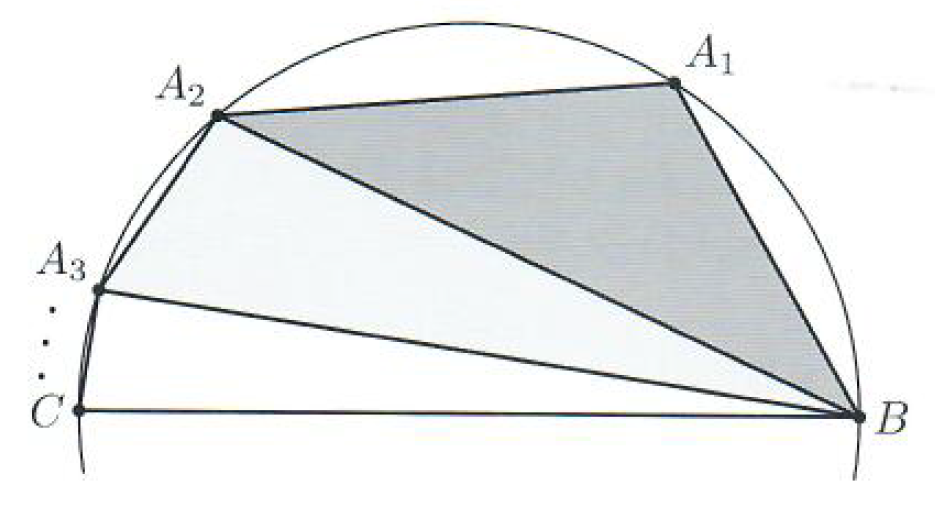
\includegraphics[width=0.4\textwidth]{2018_G3}
\end{figure}


We proceed by showing that no $t > 4$ satisfies the conditions of the problem.  To this end, we assume that there exists a good collection $T$ of $n$ triangles, each of perimeter greater than $t$, and then bound $n$ from above.

Take $\epsilon > 0$ such that $t  = 4 + 2\epsilon$.

\textit{Claim: } There exists a positive constant $\sigma = \sigma(\epsilon)$ such that any triangle $\Delta$ with perimeter $2s \geq 4 + 2\epsilon$
; inscribed in $\omega$; has area $S(\Delta)$ at least $\sigma$.

\textit{Proof:} Let $a, b, c$ be the side lengths of $\Delta$. Since $\Delta$ is inscribed in $\omega$, each side has length at most 2.  Therefore, $s-a \geq (2 + \epsilon) - 2= \epsilon$.  Similarly, $s-b \geq \epsilon$ and $s - c \geq \epsilon$.  By Heron's formula, $S(\Delta) = \sqrt{s(s-a)(s-b)(s-c)} \geq \sqrt{(2 + \epsilon) \epsilon^3}$. Thus, we can set $\sigma(\epsilon) = \sqrt{(2 + \epsilon) \epsilon^3}$. \qed \\

Now we see that the total area $S$ of all triangles from $T$ is at least $n \sigma(\epsilon)$.  On the other hand, $S$ does not exceed the area of the disk bounded by $\omega$.  Thus $n \sigma(\epsilon) \leq \pi$, which means that $n$ is bounded from above. \\

\textbf{Comment 1.}  One may prove the Claim using the formula $S  = \frac{abc}{4R}$ instead of Heron's formula. \\

\textbf{Comment 2.}  In the statement of the problem condition (i) could be replaced by a weaker one; each triangle from $T$ lies within $\omega$. This does not affect the solution above, but reduces the number of ways to prove the Claim.



\vspace{5mm}

% 2018 shortlist A5
\item[3.]  \textit{Determine all functions $f : \left(0,\infty\right) \to \mathbb{R}$ satisfying
\begin{equation} \label{a51}
    \left(x+\frac{1}{x}\right) f(y) = f\left(xy\right) +f\left(\frac{y}{x}\right)
\end{equation} 
for all $x,y > 0$. 
}
 \vspace{5mm}

\textbf{Answer: } $f(x) = C_1 x + \frac{C_2}{x}$ with arbitrary constants $C_1$ and $C_2$. \\

\textbf{Solution 1: } Fix a real number $a > 1$, and take a new variable $t$. For the values $f(t), f(t^2)$, $f(at)$, and $f(a^2 t^2)$, the given relation provides a system of linear equations:

\begin{align}
    x = y = 1: \hspace{7.4mm} \qquad \left(t + \frac{1}{t} \right) f(t) &= f(t^2) + f(1) \label{a52a} \\
    x = \frac{t}{a}, y = at:  \hspace{3.5mm} \qquad \left( \frac{t}{a} + \frac{a}{t} \right)  f(at) &= f(t^2) + f(a^2) \label{a52b} \\
    x = a^2t, y = t:  \qquad  \left( a^2t + \frac{1}{a^2t}  \right) f(t) &= f(a^2t^2) + f\left( \frac{1}{a^2}  \right) \label{a52c} \\
    x = y = at: \hspace{1mm} \qquad \left( at + \frac{1}{at}  \right) f(at) &= f(a^2 t^2) + f(1) \label{a52d}
\end{align}

In order to eliminate $f(t^2)$, take the difference of (\ref{a52a}) and (\ref{a52b}); from (\ref{a52c}) and (\ref{a52d}) eliminate $f(a^2 t^2)$; then by taking a linear combination, eliminate $f(at)$ as well:

\begin{align*}
    \left(t + \frac{1}{t} \right) f(t) - \left(\frac{t}{a} + \frac{a}{t} \right) f(at) &= f(1) - f(a^2) \quad \textrm{and} \\
    \left(a^2 t + \frac{1}{a^2 t} \right) f(t)  - \left(at + \frac{1}{at} \right) f(at) &= f(1/a^2) - f(1), \quad \textrm{so} 
\end{align*}
\begin{align*}
    ( \left(at + \frac{1}{at} \right) \left(t + \frac{1}{t} \right) &- \left(\frac{t}{a} + \frac{a}{t} \right) \left(a^2t + \frac{1}{a^2 t} \right) ) f(t) \\
    &= \left(at + \frac{1}{at} \right) (f(1) - f(a^2)) - \left(\frac{t}{a} + \frac{a}{t} \right) (f(1/a^2) - f(1)).
\end{align*}

Notice that on the left-hand side, the coefficient of $f(t)$ is nonzero and does not depend on $t$:
\begin{equation*}
    \left(at + \frac{1}{at} \right) \left(t + \frac{1}{t} \right) - \left(\frac{t}{a} + \frac{a}{t} \right) \left(a^2t + \frac{1}{a^2 t} \right) = a + \frac{1}{a} - \left(a^3 + \frac{1}{a^3} \right) < 0
\end{equation*}

After dividing by this fixed number, we get
\begin{equation} \label{a53}
    f(t) = C_1 t + \frac{C_2}{t} 
\end{equation}

where the numbers $C_1$ and $C_2$ are expressed in terms of $a$, $f(1)$, $f(a^2)$, and $f(1/a^2)$, and they do not depend on $t$.

The functions of the form (\ref{a53}) satisfy the equation:
$$
\left( x + \frac{1}{x} \right) f(y) = \left( x + \frac{1}{x} \right) \left( C_1 y + \frac{C_2}{y} \right) = \left( C_1 xy + \frac{C_2}{xy} \right) + \left(C_1 \frac{y}{x} + C_2 \frac{x}{y} \right) = f(xy) + f\left( \frac{y}{x} \right)
$$ \\


\textbf{Solution 2:}  We start with an observation.  If we substitute $x = a \not = 1$ and $y = a^n$ in the given, we obtain
$$
f(a^{n+1}) - \left(a + \frac{1}{a} \right)  f(a^n) + f(a^{n-1}) = 0
$$

For the sequence $z_n = a^n$, this is a homogeneous linear recurrence of the second order, and its characteristic polynomial is $t^2 - (a + \frac{1}{a})t + 1 = (t-a)(t - \frac{1}{a})$ with two distinct nonzero roots, namely $a$ and $1/a$. As is well-known, the general solution is $z_n = C_1 a^n + C_2 (1/a)^n$ where the index $n$ can be as well positive as negative. Of course, the numbers $C_1$ and $C_2$ may depend of the choice of $a$, so in fact we have two functions, $C_1$ and $C_2$, such that
\begin{equation} \label{a54}
    f(a^n) = C_1(a) \cdot a^n + \frac{C_2(a)}{a^n} \quad \textrm{for every $a \not = 1$ and every integer $n$}
\end{equation}

The relation (\ref{a54}) can be easily extended to rational values of $n$, so we may conjecture that $C_1$ and $C_2$ are constants, and whence $f(t) = C_1 t + \frac{C_2}{t}$.  As it was seen in the previous solution, such functions indeed satisfy the given.

The equation (\ref{a51}) is linear in $f$; so if some functions $f_1$ and $f_2$ satisfy (\ref{a51}) and $c_1, c_2$ are real numbers, then $c_1 f_1(x) + c_2 f_2(x)$ is also a solution of (\ref{a51}). In order to make our formulas simpler, define
$ f_0(x) = f(x) - f(1) \cdot x$.

This function is another one satisfying (\ref{a51}) and the extra constraint $f_0(1) = 0$. Repeating the same argument on linear recurrences, we can write $f_0(a) = K(a) a^n + \frac{L(a)}{a^n}$ with some functions $K$ and $L$. By substituting $n = 0$, we can see that $K(a) + L(a) = f_0(1) = 0$ for every $a$. Hence,

$$
f_0(a^n) = K(a) \left( a^n - \frac{1}{a^n}  \right)
$$

Now take two numbers $a > b > 1$ arbitrarily and substitute $x = (a/b)^n$ and $y = (ab)^n$ in (\ref{a51}):

\begin{align}
    \left(\frac{a^n}{b^n} + \frac{b^n}{a^n} \right) f_0((ab)^n) &= f_0(a^{2n}) + f_0(b^{2n}), \quad \textrm{so} \nonumber \\
    \left(\frac{a^n}{b^n} + \frac{b^n}{a^n} \right) K(ab) \left((ab)^n + \frac{1}{(ab)^n} \right) &= K(a) \left(a^{2n} - \frac{1}{a^{2n}} \right) + K(b) \left(b^{2n} - \frac{1}{b^{2n}} \right), \quad \textrm{or equivalently} \nonumber \\
    K(ab) \left( a^{2n} - \frac{1}{a^{2n}} + b^{2n} - \frac{1}{b^{2n}}    \right) &= K(a) \left(a^{2n} - \frac{1}{a^{2n}} \right) + K(b) \left(b^{2n} - \frac{1}{b^{2n}} \right) \label{a55}.
\end{align}

By dividing (\ref{a55}) by $a^{2n}$ and then taking limit with $n \to + \infty$, we get $K(ab) = K(a)$. Then (\ref{a55}) reduced to $K(a) = K(b)$. Hence, $K(a) = K(b)$ for all $a > b > 1$.

Fix $a > 1$. For every $x > 0$, there is some $b$ and an integer $n$ such that $1 < b < a$ and $x = b^n$. Then
$$
f_0(x) = f_0(b^n) = K(b) \left(b^n - \frac{1}{b^n} \right) = K(a) \left(  x  - \frac{1}{x} \right).
$$

Hence, we have $f(x) = f_0(x) + f(1)x = C_1 x + \frac{C_2}{x}$ with $C_1 = K(a) + f(1)$ and $C_2 = -K(a)$. \\

\textbf{Comment:}  After establishing (\ref{a55}), there are several variants of finishing the solution.  For example, instead of taking a limit, we can obtain a system of linear equations for $K(a)$, $K(b)$, and $K(ab)$ by substituting two positive integers $n$ in (\ref{a55}), say $n = 1$ and $n = 2$. This approach leads to a similar ending as in the first solution.

Optionally, we define another function $f_1(x) = f_0(x) - C(x - \frac{1}{x})$ and prescribe $K(c) = 0$ for another fixed $c$. Then we can choose $ab = c$ and decrease the number of terms in (\ref{a55}).

\vspace{6mm}


    

\end{enumerate}
\end{document}




